\documentclass{beamer}

\mode<presentation>
{
\usetheme{Madrid}
}

\usepackage{graphics, graphicx}
\usepackage{booktabs}
\DeclareGraphicsExtensions{.pdf,.png,.jpg,.gif}

\title{Linux Beginner Guide}

\author{Jaewoong Lee}

\institute[UNIST]
{
	Ulsan National Institute of Science and Technology
	\medskip
	\newline
	\textit{jwlee230@unist.ac.kr}
}

\date{\today}

\begin{document}
	\begin{frame}
		\titlepage
	\end{frame}

	\begin{frame}
		\frametitle{Introduction}
		
		In this guide, I assume that followings are already installed:
		\begin{enumerate}
			\item Ubuntu 16.04.2 or Higher
			\item ZSH 5.0.2 or Higher
			\item VIM 8.1 or Higher
			\item We will connect to server via SSH
		\end{enumerate}

		With this guide, you can use and understand Linux system. \\
		Also, this guide includes as little information about operating system as possible. If you find some fault in the strict sense of the word, that means you are not \textbf{beginner}. 
	\end{frame}

	\begin{frame}
		\frametitle{Overview}
		\tableofcontents
	\end{frame}

	\section{Linux?}
	
	\begin{frame}
		\frametitle{Linux?}
		\begin{figure}[h!]
			\centering
			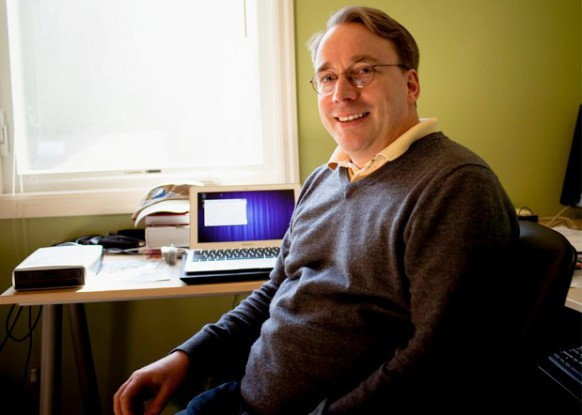
\includegraphics[width=0.4 \linewidth]{figures/linus.jpg}
			\caption{Linus Torvalds, Inventor of Linux}
		\end{figure}
	
		Linux is one of the most famous OS as Windows and macOS. \\
		Linux is open-source project. \\
		Android, OS for mobile, is based on Linux. 
	\end{frame}

	\begin{frame}
		\frametitle{Ubuntu?}
		\begin{figure}[h!]
			\centering
			
\includegraphics[width=0.3 \linewidth]{figures/ubuntu.jpg}
			\caption{Logo of Ubuntu}
		\end{figure}
		Ubuntu is an OS which is based on Linux. \\
		Ubuntu is the best OS in Linux-like OS, because of convenience of its installation and usage.
	\end{frame}
	
	\section{Basic Linux Command}
	
	\begin{frame}
		\frametitle{Where we start}
		\begin{figure}[h!]
			\centering
			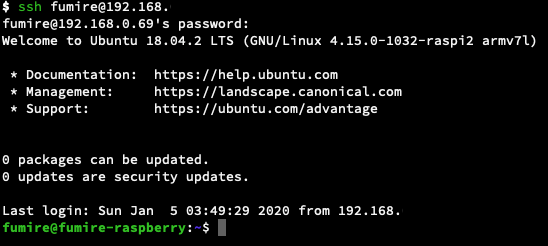
\includegraphics[width=0.5 \linewidth]{figures/1.png}
			\caption{Here is where we start}
		\end{figure}
	
		After you connect to server via SSH, you can see like this. \\
		Here is where we start! \\
		\textit{fumire} will be user name, and \textit{fumire-raspberry} will be server name. 
	\end{frame}

	\begin{frame}
		\frametitle{pwd}
		\begin{figure}[h!]
			\centering
			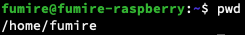
\includegraphics[width=0.5 \linewidth]{figures/2.png}
			\caption{Result of \textit{pwd} Command}
		\end{figure}
		\textit{pwd} is abbr. of "Print Working Directory". \\
		You can see where you are with \textit{pwd} command. \\
		Also, "/home/username" is your \textit{home folder}.
	\end{frame}

	\begin{frame}
		\frametitle{ls}
		\begin{figure}[h!]
			\centering
			
\includegraphics[width=0.7 \linewidth]{figures/3.png}
			\caption{Result of \textit{ls} Command}
		\end{figure}
	
		\textit{ls} stands for "List". \\
		\textit{ls} command lists current directory contents. \\
		If current directory is empty, the result will be nothing. 
	\end{frame}

	\begin{frame}
		\frametitle{Configuration}
		However, you have not completed configuration. Therefore, finish settings with following command:
		\begin{example}
			\$ git clone https://github.com/Fumire/.dotfiles.git \\
			\$ cd .dotfiles \\
			\$ make \\
			\$ chsh -s /usr/bin/zsh
		\end{example}
		Note that you should input command only after '\$'. \\
		After executing commands, you should restart your shell. 
	\end{frame}

	\begin{frame}
		\frametitle{Configuration \textit{(Cont.)}}
		\begin{figure}[h!]
			\centering
			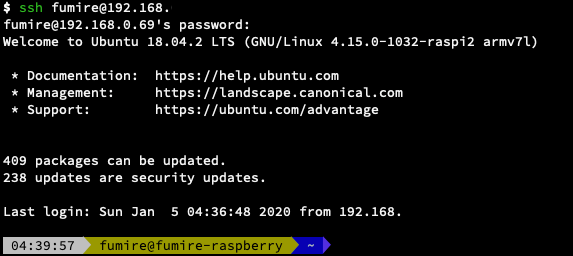
\includegraphics[width=0.7 \linewidth]{figures/4.png}
			\caption{ZSH}
		\end{figure}
	
		With successful configuration, you can see like this. 
	\end{frame}
	
	\section{Edit File with VIM}
	
	\section{How to Download from Web}
	
	\section{User Permissions}
	
	\section{IO Redirections}
	
	\section{Process Control}
	
	\section{Process Control with SGE}

\end{document}